\documentclass[t]{beamer}
\usepackage{helvet}
\usepackage{calc}
\usepackage[utf8]{inputenc} % set your input encoding differently, if you want
\usepackage[english]{babel}

% Setting style of presentation
% =============================
\usetheme{Boadilla}
%\setbeamercovered{transparent=10}
%\setbeamertemplate{navigation symbols}{}


% Some common packages
% ====================
\usepackage{units}
\usepackage{amsbsy}
\usepackage{amsmath}
\usepackage{amssymb}
\usepackage{graphics}
\usepackage{epsf}
\usepackage{epsfig}
\usepackage{fixmath}
\usepackage{wrapfig}
\usepackage{tcolorbox}

\usepackage{bytefield}

\usepackage{array}
\newcolumntype{M}{>{\centering\arraybackslash}m{\dimexpr.25\linewidth-2\tabcolsep}}

% Adapt title information
% =======================
\title{Development of a temperature sensor network\\for the nEDM experiment}
\author{Wenwen Chen, Rainer Schönberger}
%\institute{Department for Computer Science\\Technische Universität München}
\date{\today}





% ==============
% DOCUMENT BEGIN
% ==============
\begin{document}

% Typeset title page
% ------------------------------------------------------------------------
%\setbeamertemplate{background}{\NETBlackTransparent{width=2.3\paperwidth}}
\begin{frame}
    \titlepage
\end{frame}
%\setbeamertemplate{background}{}
% ------------------------------------------------------------------------

% Outline
% ------------------------------------------------------------------------
%\begin{frame}
%    \frametitle{Outline}
%    \tableofcontents
%\end{frame}
% ------------------------------------------------------------------------



% MOTIVATION
% ------------------------------------------------------------------------
\begin{frame}[c]
    \frametitle{Requirements}
		\begin{alertblock}{Must}
			\begin{itemize}
				\item Temperature and humidity measurement
				\item High accuracy: $\pm0.1\mathrm{K}$
				\item High number of sensors: $\approx$ 40
        \item Low cost
				\item Send results to couchDB
        \item Ready to use 
				\item Reliable and stable
			\end{itemize}
		\end{alertblock}
\end{frame}
\begin{frame}[c]
    \frametitle{Requirements}
		\begin{exampleblock}{May}
			\begin{itemize}
				\item Extendible
        \item Easy maintenance
				\item Plug and Play
				\item Sample interval $\le 1\mathrm{s}$
				\item Easy configuration at runtime
			\end{itemize}
		\end{exampleblock}
\end{frame}
\begin{frame}[c]
    \frametitle{Components structure}
  \begin{center}
  	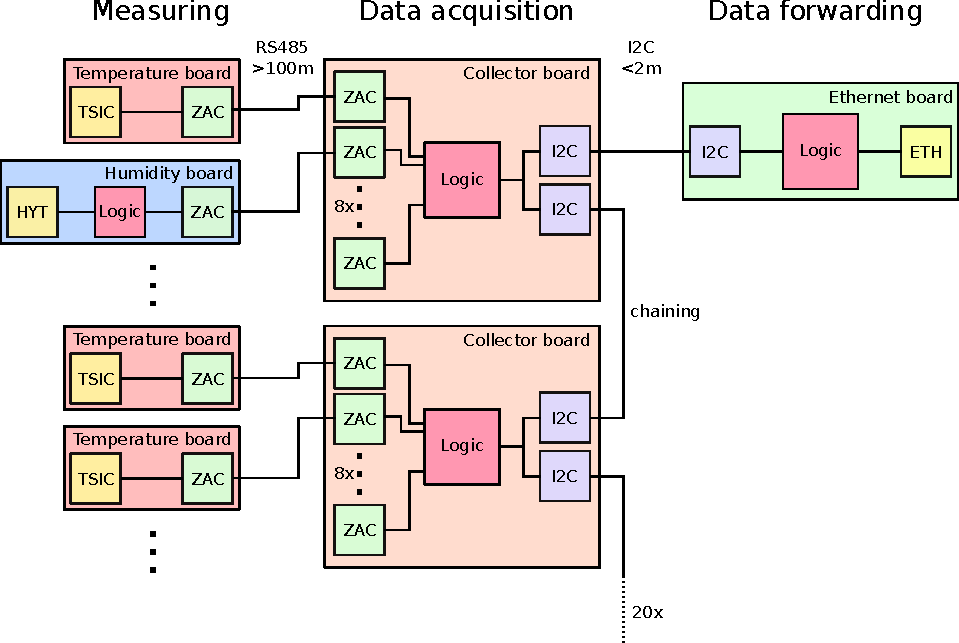
\includegraphics[width=0.9\linewidth]{img/plan2_color.pdf}\\
  \vspace{0.5cm}
  \end{center}
\end{frame}
\begin{frame}[c]
    \frametitle{Hardware}
\begin{tabular}{ M M M M}
	Sensor & Accuracy & Resolution & Cost\tabularnewline
	\hline
	\hline
	TSIC 506F& $\pm 0.1\mathrm{K}$ & $\pm 0.034\mathrm{K}$ & $8 \mathrm{EUR}$\tabularnewline
	\hline
	HYT271 & $\pm 1.8\mathrm{\%RH}$ & $\pm 0.03\mathrm{\%RH}$ & $20 \mathrm{EUR}$\tabularnewline
	& $\pm 0.2\mathrm{K}$ & $\pm 0.015\mathrm{K}$ & \tabularnewline
	\hline
\end{tabular}
\end{frame}
\begin{frame}[c]
    \frametitle{Proof of concept}
  \begin{center}
  	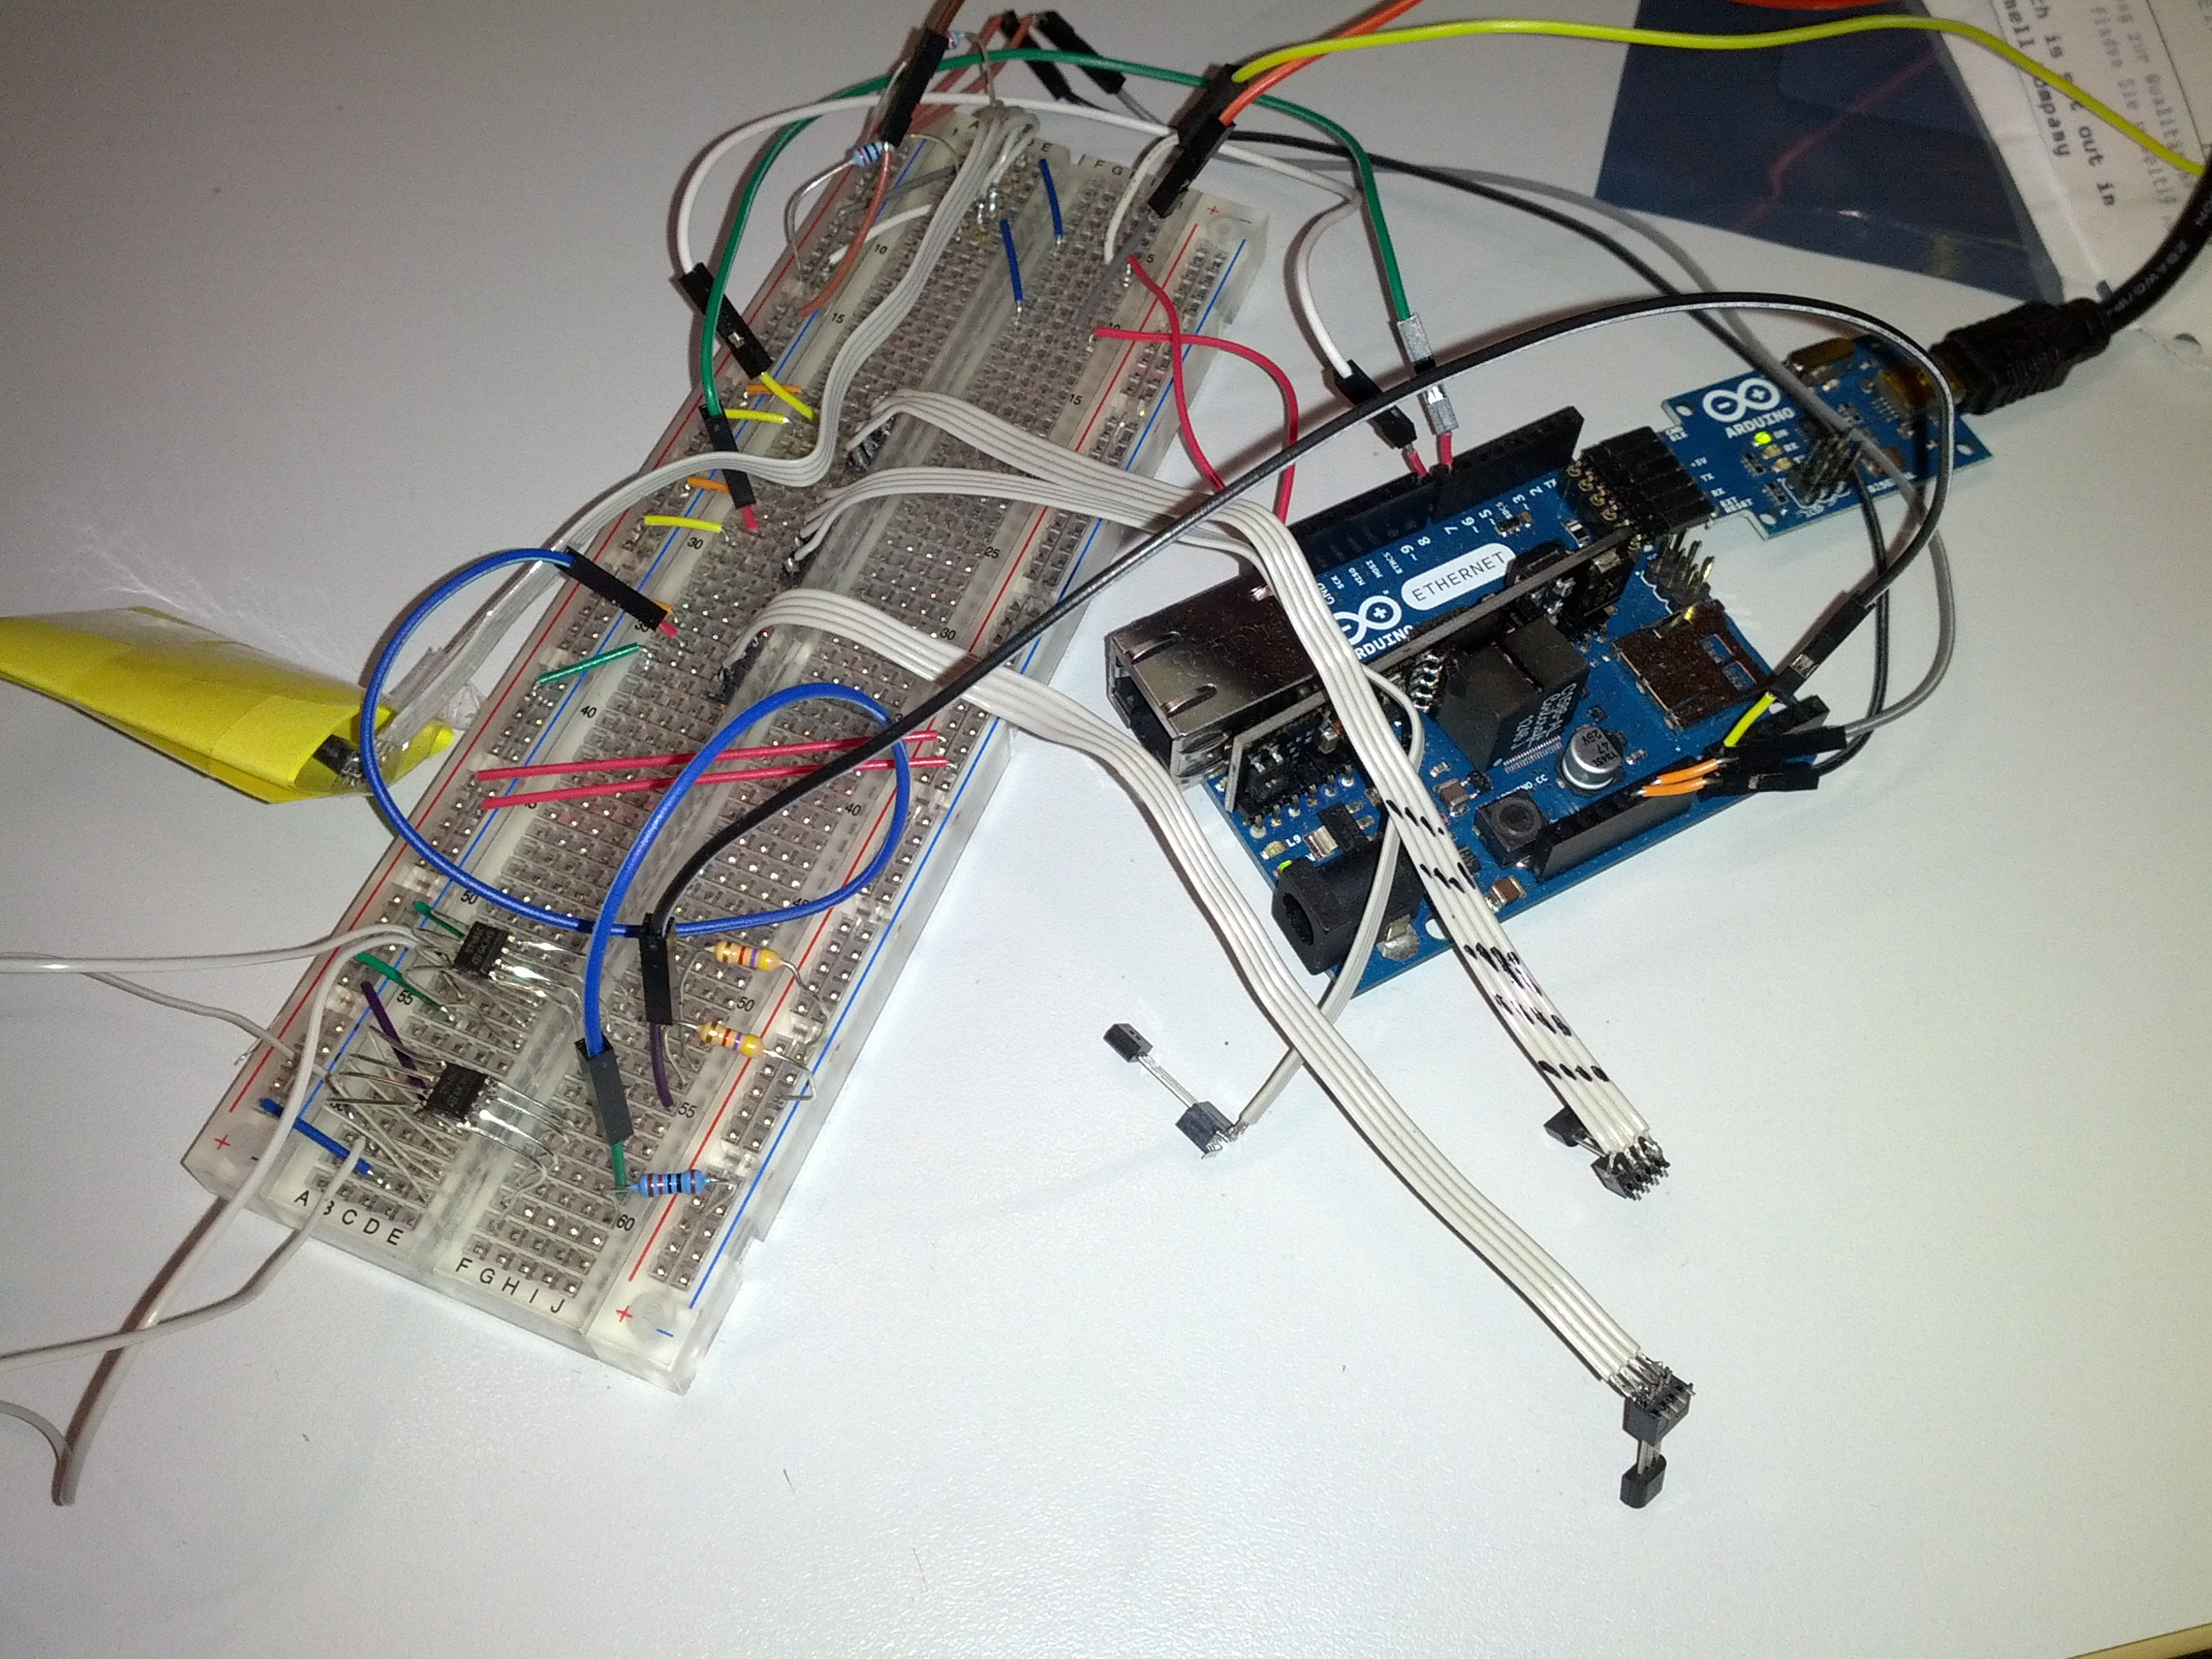
\includegraphics[width=0.8\linewidth]{img/pic/IMG_20140410_213954.jpg}\\
  \vspace{0.5cm}
  \end{center}
\end{frame}
\begin{frame}[c]
    \frametitle{First load of PCBs arrived}
  \begin{center}
  	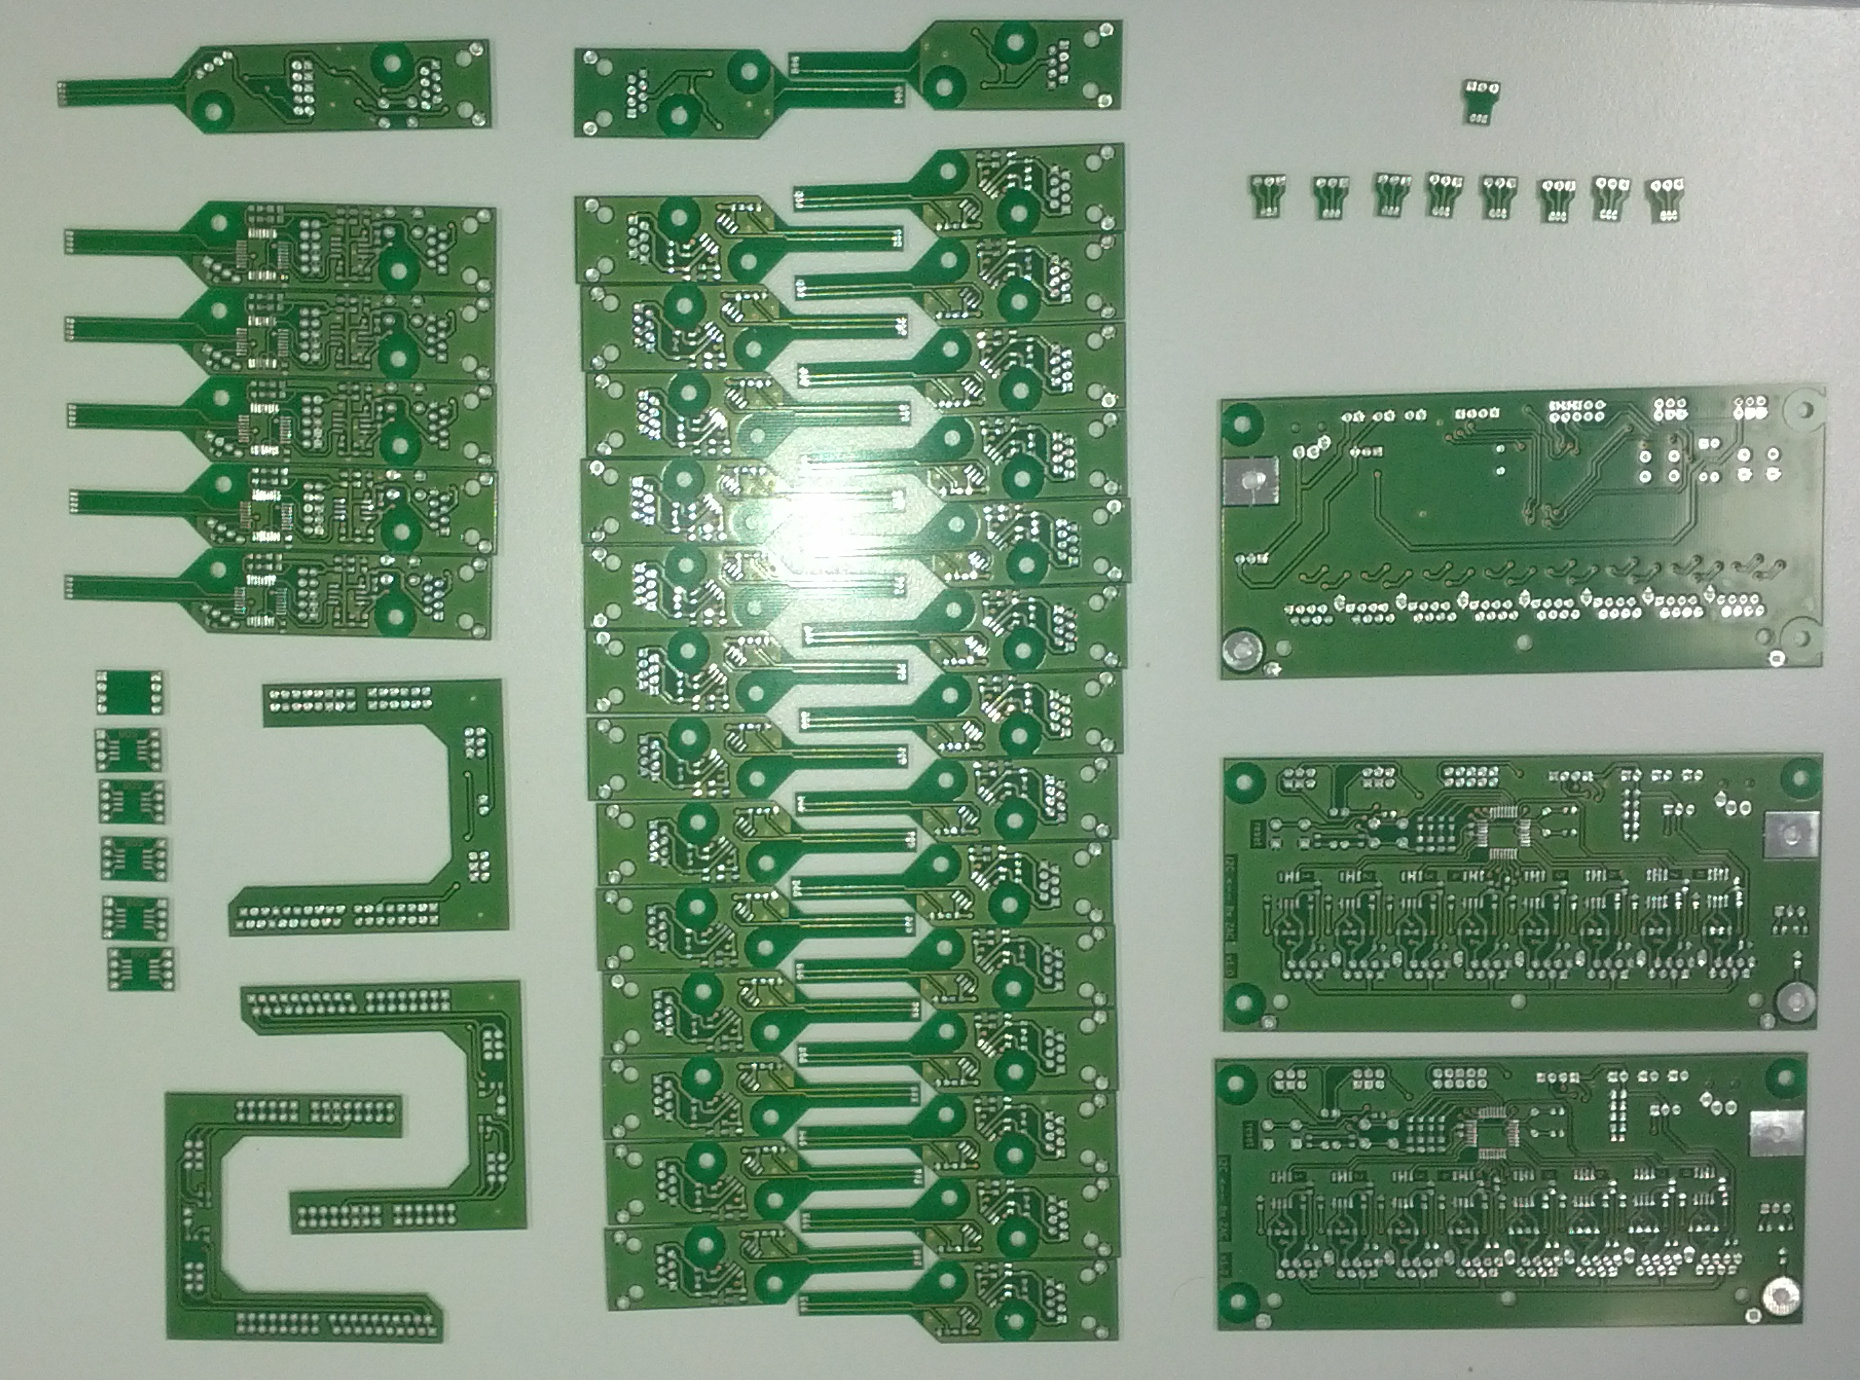
\includegraphics[width=0.8\linewidth]{img/pic/platinen_leer.jpg}\\
  \vspace{0.5cm}
  \end{center}
\end{frame}
\begin{frame}[c]
    \frametitle{Hours of soldering later...}
  \begin{center}
  	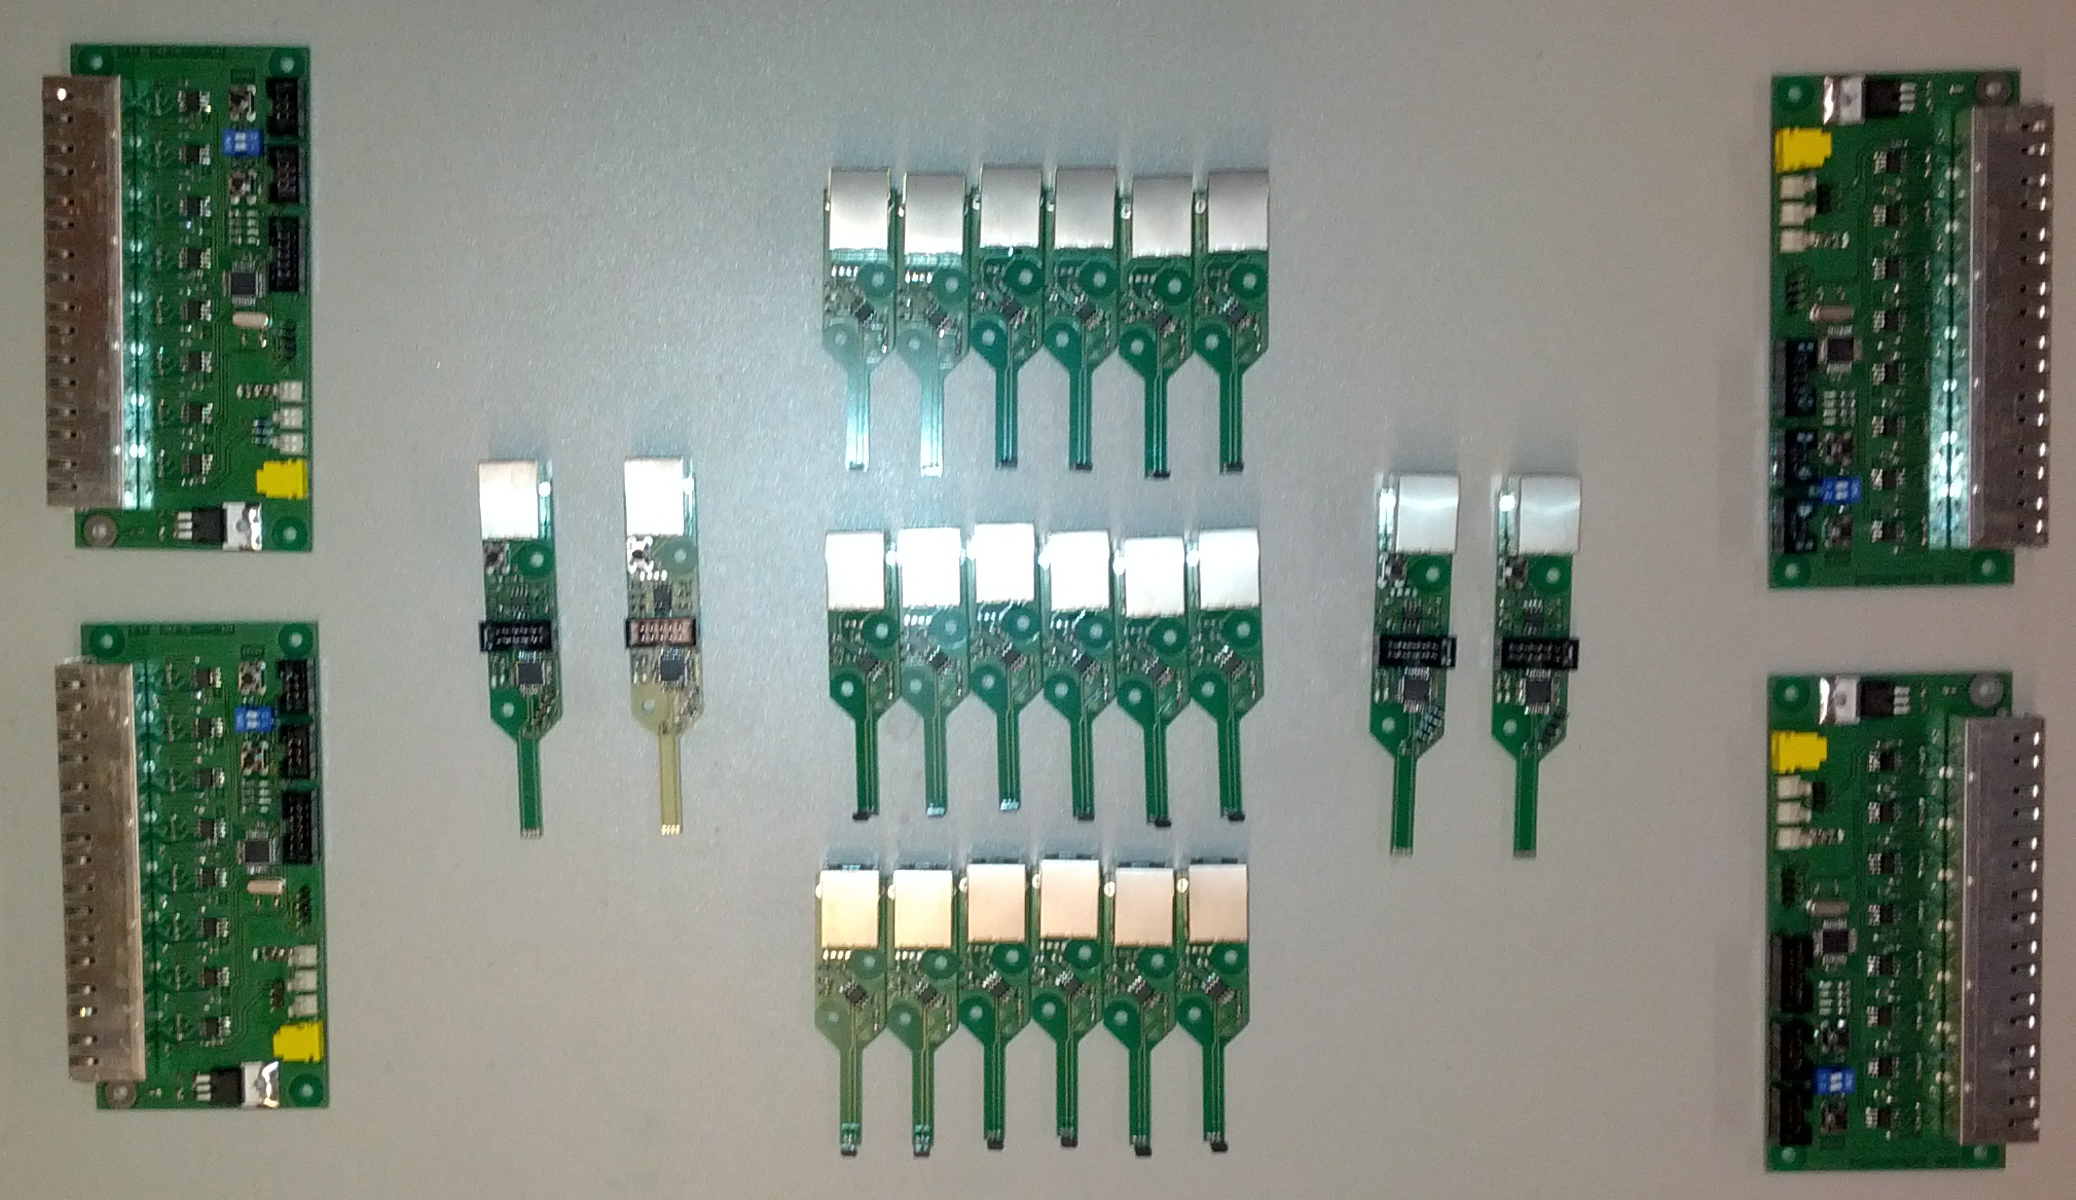
\includegraphics[width=0.8\linewidth]{img/pic/platinen_geloetet.jpg}\\
  \vspace{0.5cm}
  \end{center}
\end{frame}
\begin{frame}[c]
    \frametitle{Collector board}
  \begin{center}
  	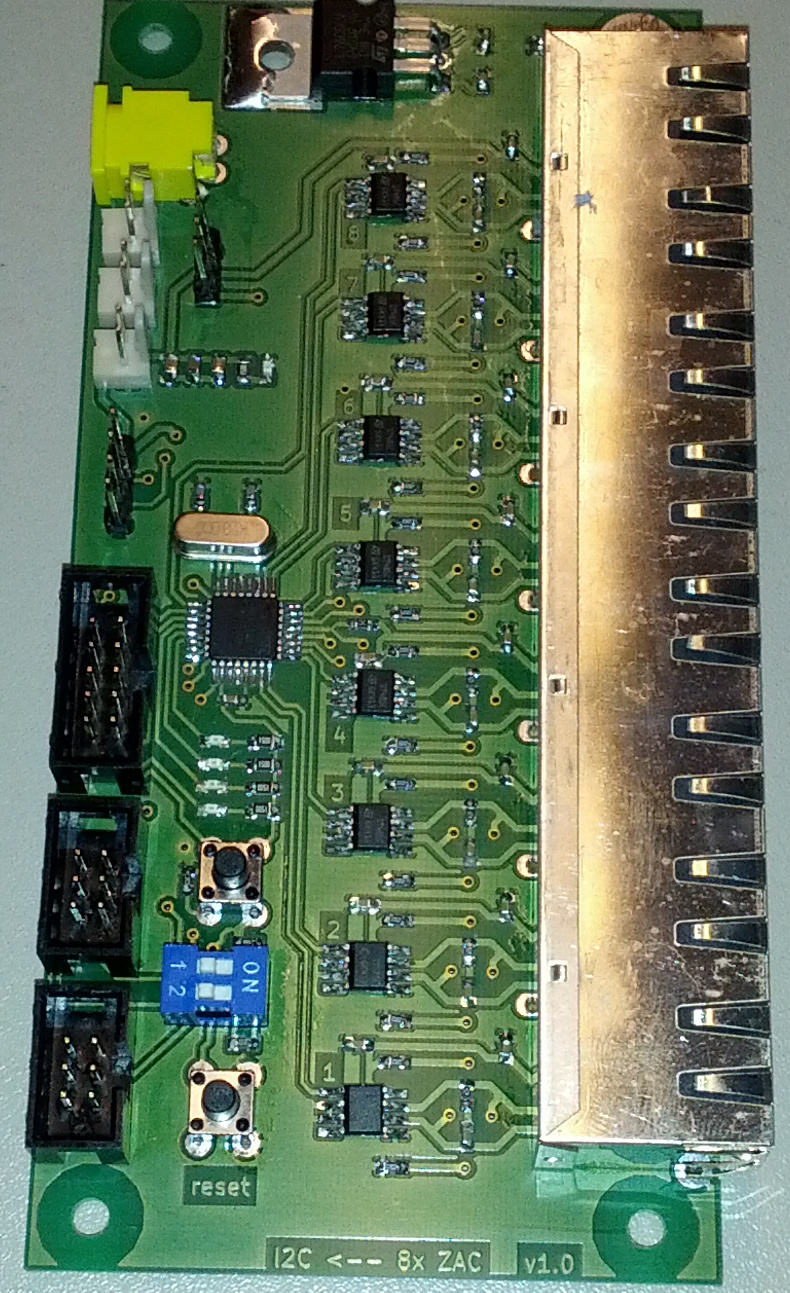
\includegraphics[width=0.4\linewidth]{img/pic/collector_geloetet.jpg}\\
  \vspace{0.5cm}
  \end{center}
\end{frame}
\begin{frame}[c]
    \frametitle{Material cost per board}
		\begin{description}
			\item{\textbf{Collector board:}} 20 EUR
			\item{\textbf{Temperature board:}} 12 EUR
			\item{\textbf{Humidity board:}} 30 EUR
		\end{description}
\end{frame}
\begin{frame}[c]
    \frametitle{Components structure}
  \begin{center}
  	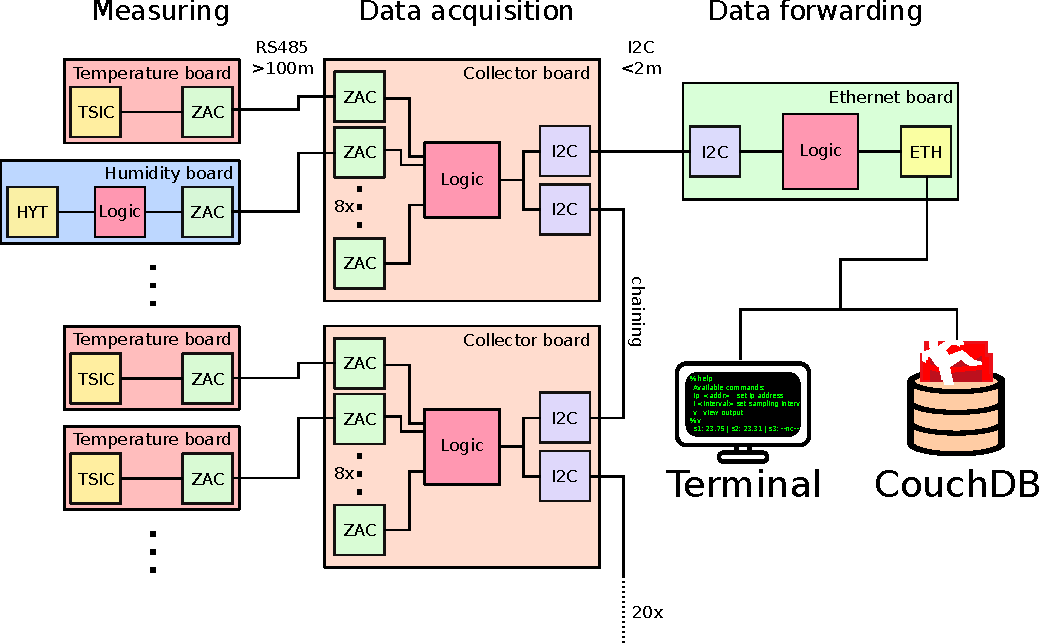
\includegraphics[width=0.9\linewidth]{img/plan2_color_db.pdf}\\
  \vspace{0.5cm}
  \end{center}
\end{frame}
\begin{frame}[c]
    \frametitle{ZAC Protocol}
  \begin{center}
  	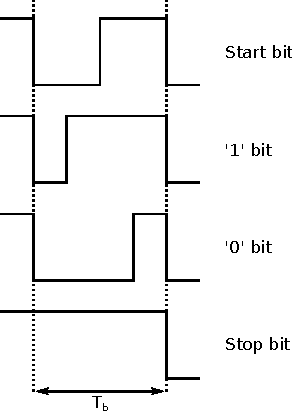
\includegraphics[width=0.4\linewidth]{img/zac_bits.pdf}\\
  \vspace{0.5cm}
  \end{center}
\end{frame}
\begin{frame}[c]
    \frametitle{ZAC Timing}
  \begin{center}
  	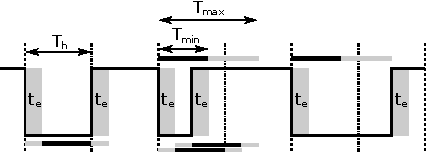
\includegraphics[width=0.8\linewidth]{img/zac_timing.pdf}\\
  \vspace{0.5cm}
  \end{center}
\end{frame}
\begin{frame}[c,fragile]
    \frametitle{I2C Protocol - Command}
  \begin{center}
	\begin{bytefield}[endianness=big, bitwidth=2em]{8}
		\bitheader{0-7}\\
		\bitbox{7}{Address} &
		\bitbox{1}{R/W}\\
		\wordbox{1}{Command}\\
		\wordbox{1}{Argument}
	\end{bytefield}
  \end{center}
\end{frame}
\begin{frame}[c,fragile]
    \frametitle{I2C Protocol - Receive}
  \begin{center}
		\begin{bytefield}[endianness=big, bitwidth=2.1em]{8}
		\bitheader{0-7}\\
		\begin{rightwordgroup}{Header}
			\bitbox{2}{type} & \bitbox{3}{\color{lightgray}\rule{\width}{\height}} & \bitbox{1}{c} & \bitbox{2}{error}
		\end{rightwordgroup}\\
		\begin{rightwordgroup}{Payload}
			\wordbox{2}{Temperature}\\
			\wordbox{2}{Humidity}
		\end{rightwordgroup}\\
		\wordbox{1}{CRC-8}
	\end{bytefield}
  \end{center}
\end{frame}
\begin{frame}[c]
    \frametitle{couchDB}
  \begin{center}
  	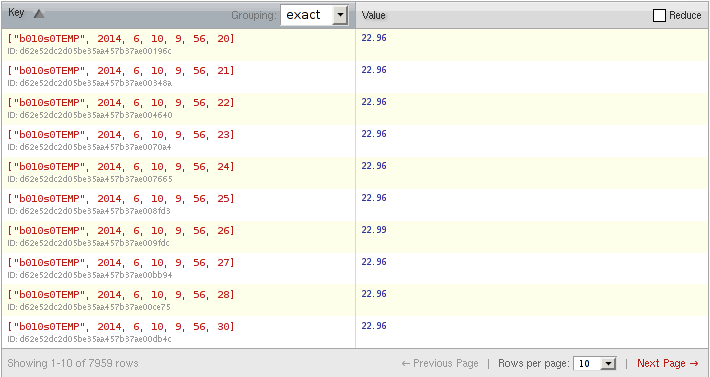
\includegraphics[width=0.9\linewidth]{img/db1.png}\\
  \vspace{0.5cm}
  \end{center}
    
\end{frame}
\begin{frame}[c]
    \frametitle{couchDB}
  \begin{center}
  	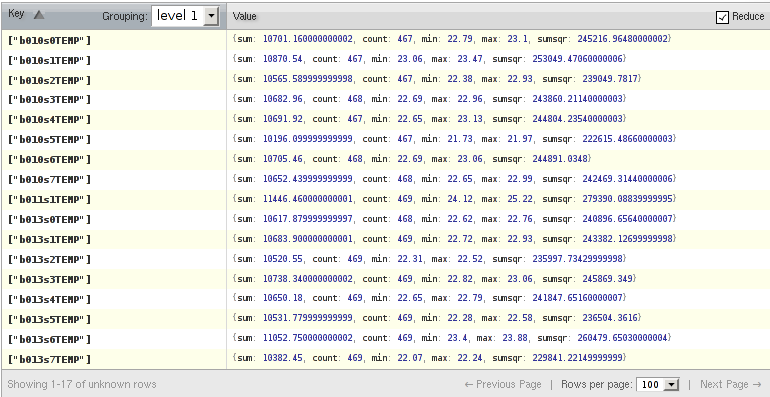
\includegraphics[width=0.9\linewidth]{img/db2.png}\\
  \vspace{0.5cm}
  \end{center}
\end{frame}
\begin{frame}[c]
    \frametitle{User interface}
  \begin{center}
  	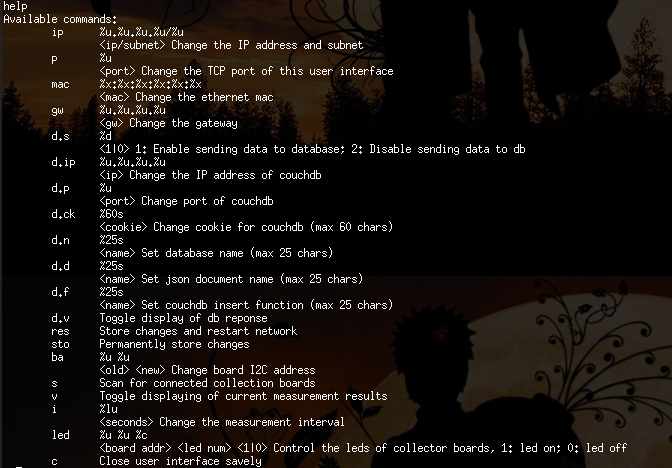
\includegraphics[width=0.9\linewidth]{img/ui.png}\\
  \vspace{0.5cm}
  \end{center}
\end{frame}
\begin{frame}[c]
    \frametitle{User interface}
  \begin{center}
  	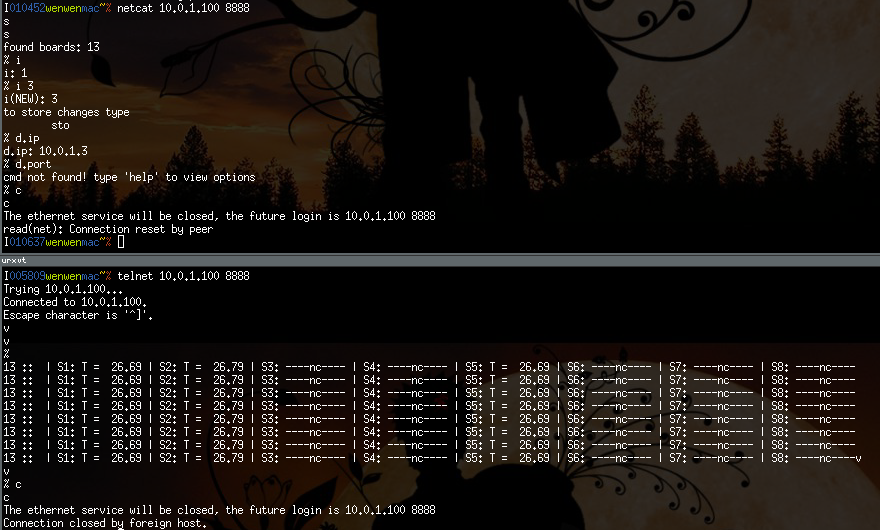
\includegraphics[width=0.9\linewidth]{img/ui2.png}\\
  \vspace{0.5cm}
  \end{center}
\end{frame}
\begin{frame}[c]
    \frametitle{Ready to install}
  \begin{center}
  	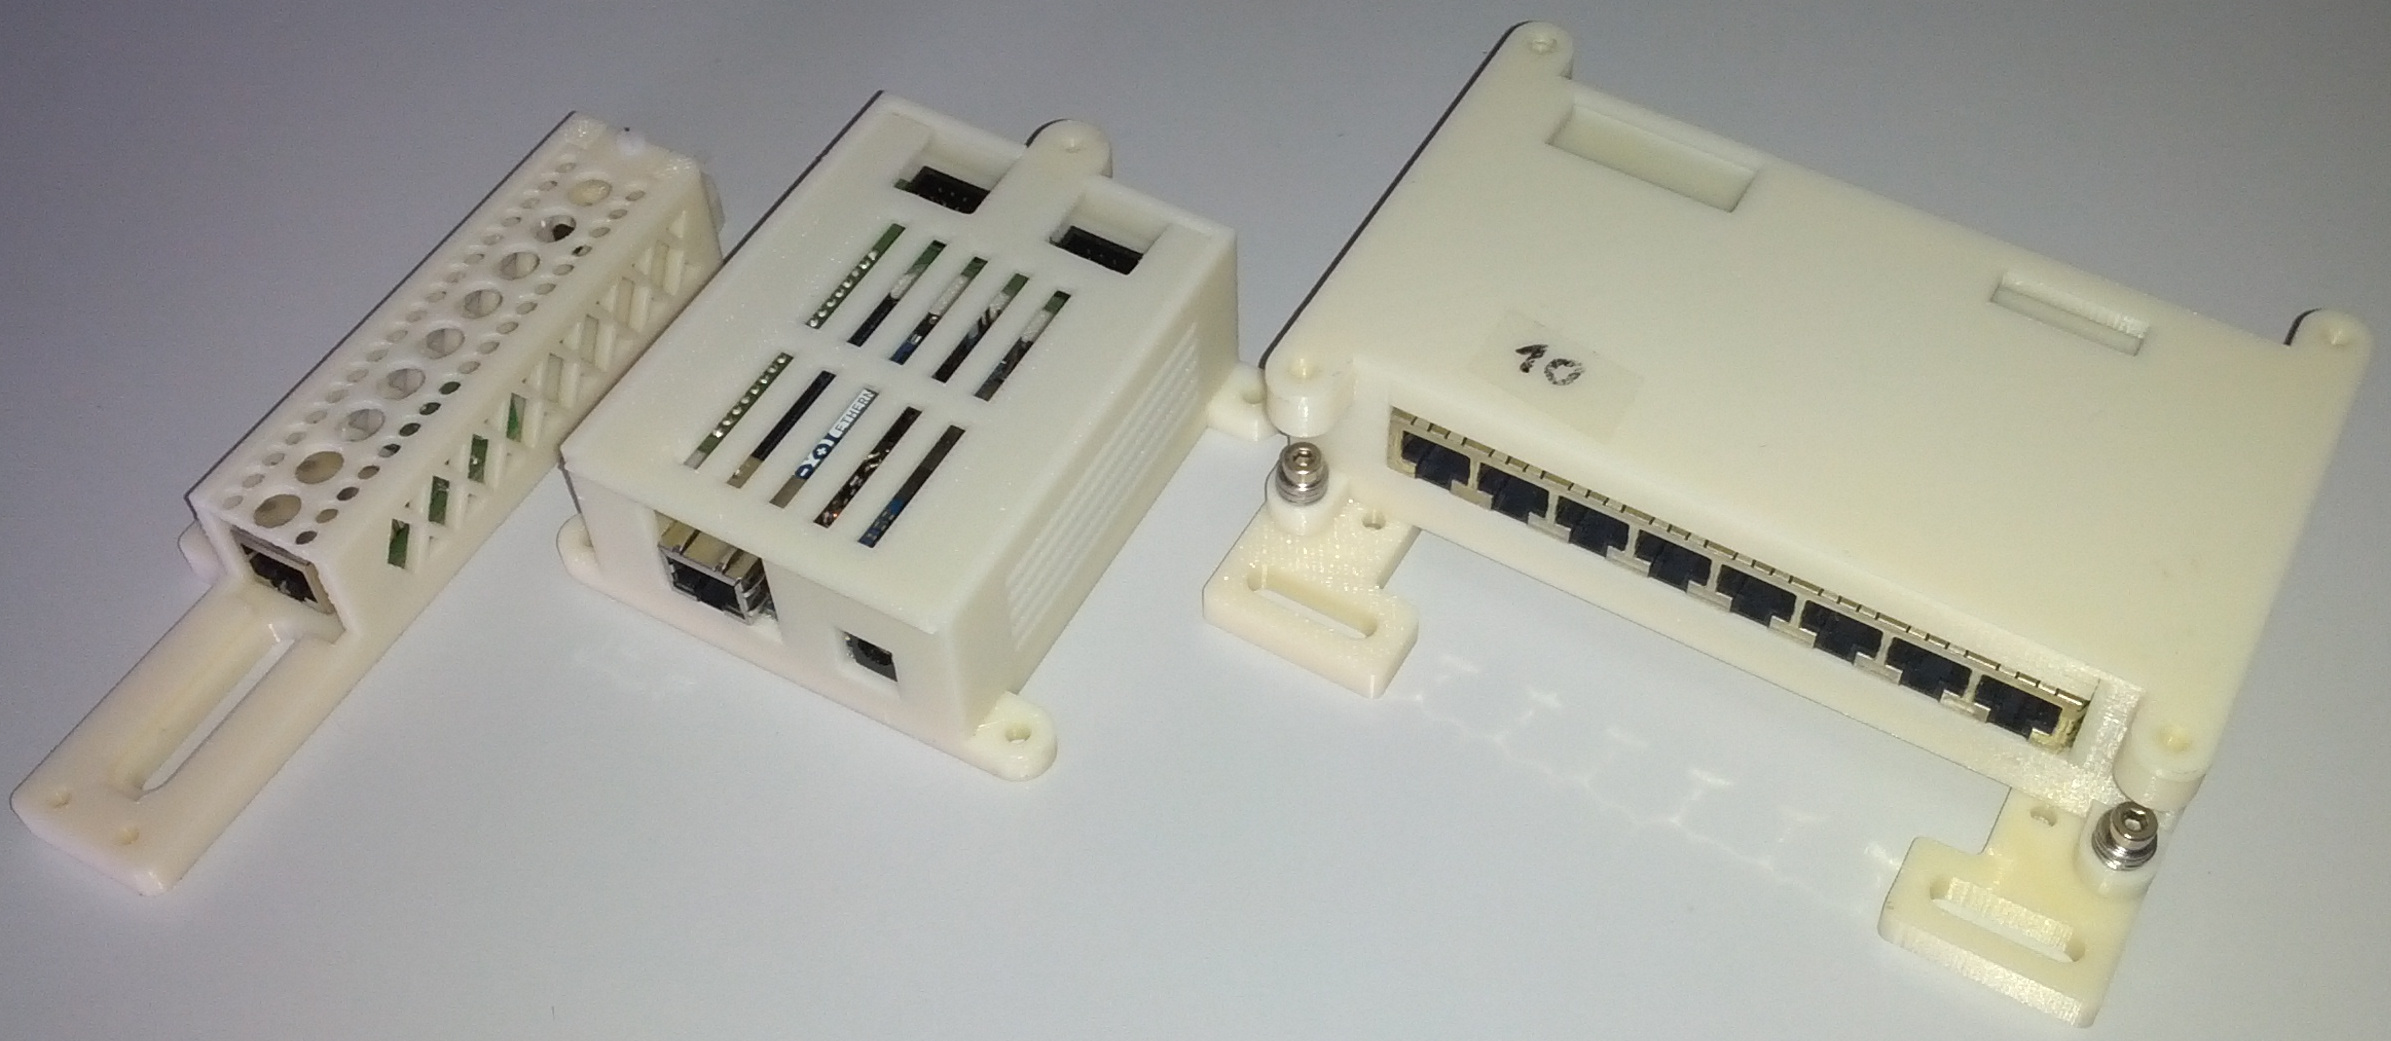
\includegraphics[width=0.9\linewidth]{img/pic/cases.jpg}\\
  \vspace{0.5cm}
  \end{center}
\end{frame}
\begin{frame}[c]
    \frametitle{Ready to install}
  \begin{center}
  	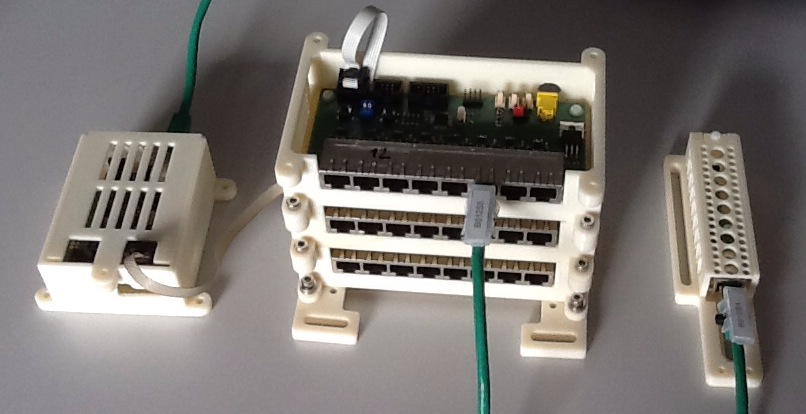
\includegraphics[width=0.9\linewidth]{img/set.jpg}\\
  \vspace{0.5cm}
  \end{center}
\end{frame}
%\begin{frame}[c]
%    \frametitle{3D - Printing}
%  \begin{center}
%  	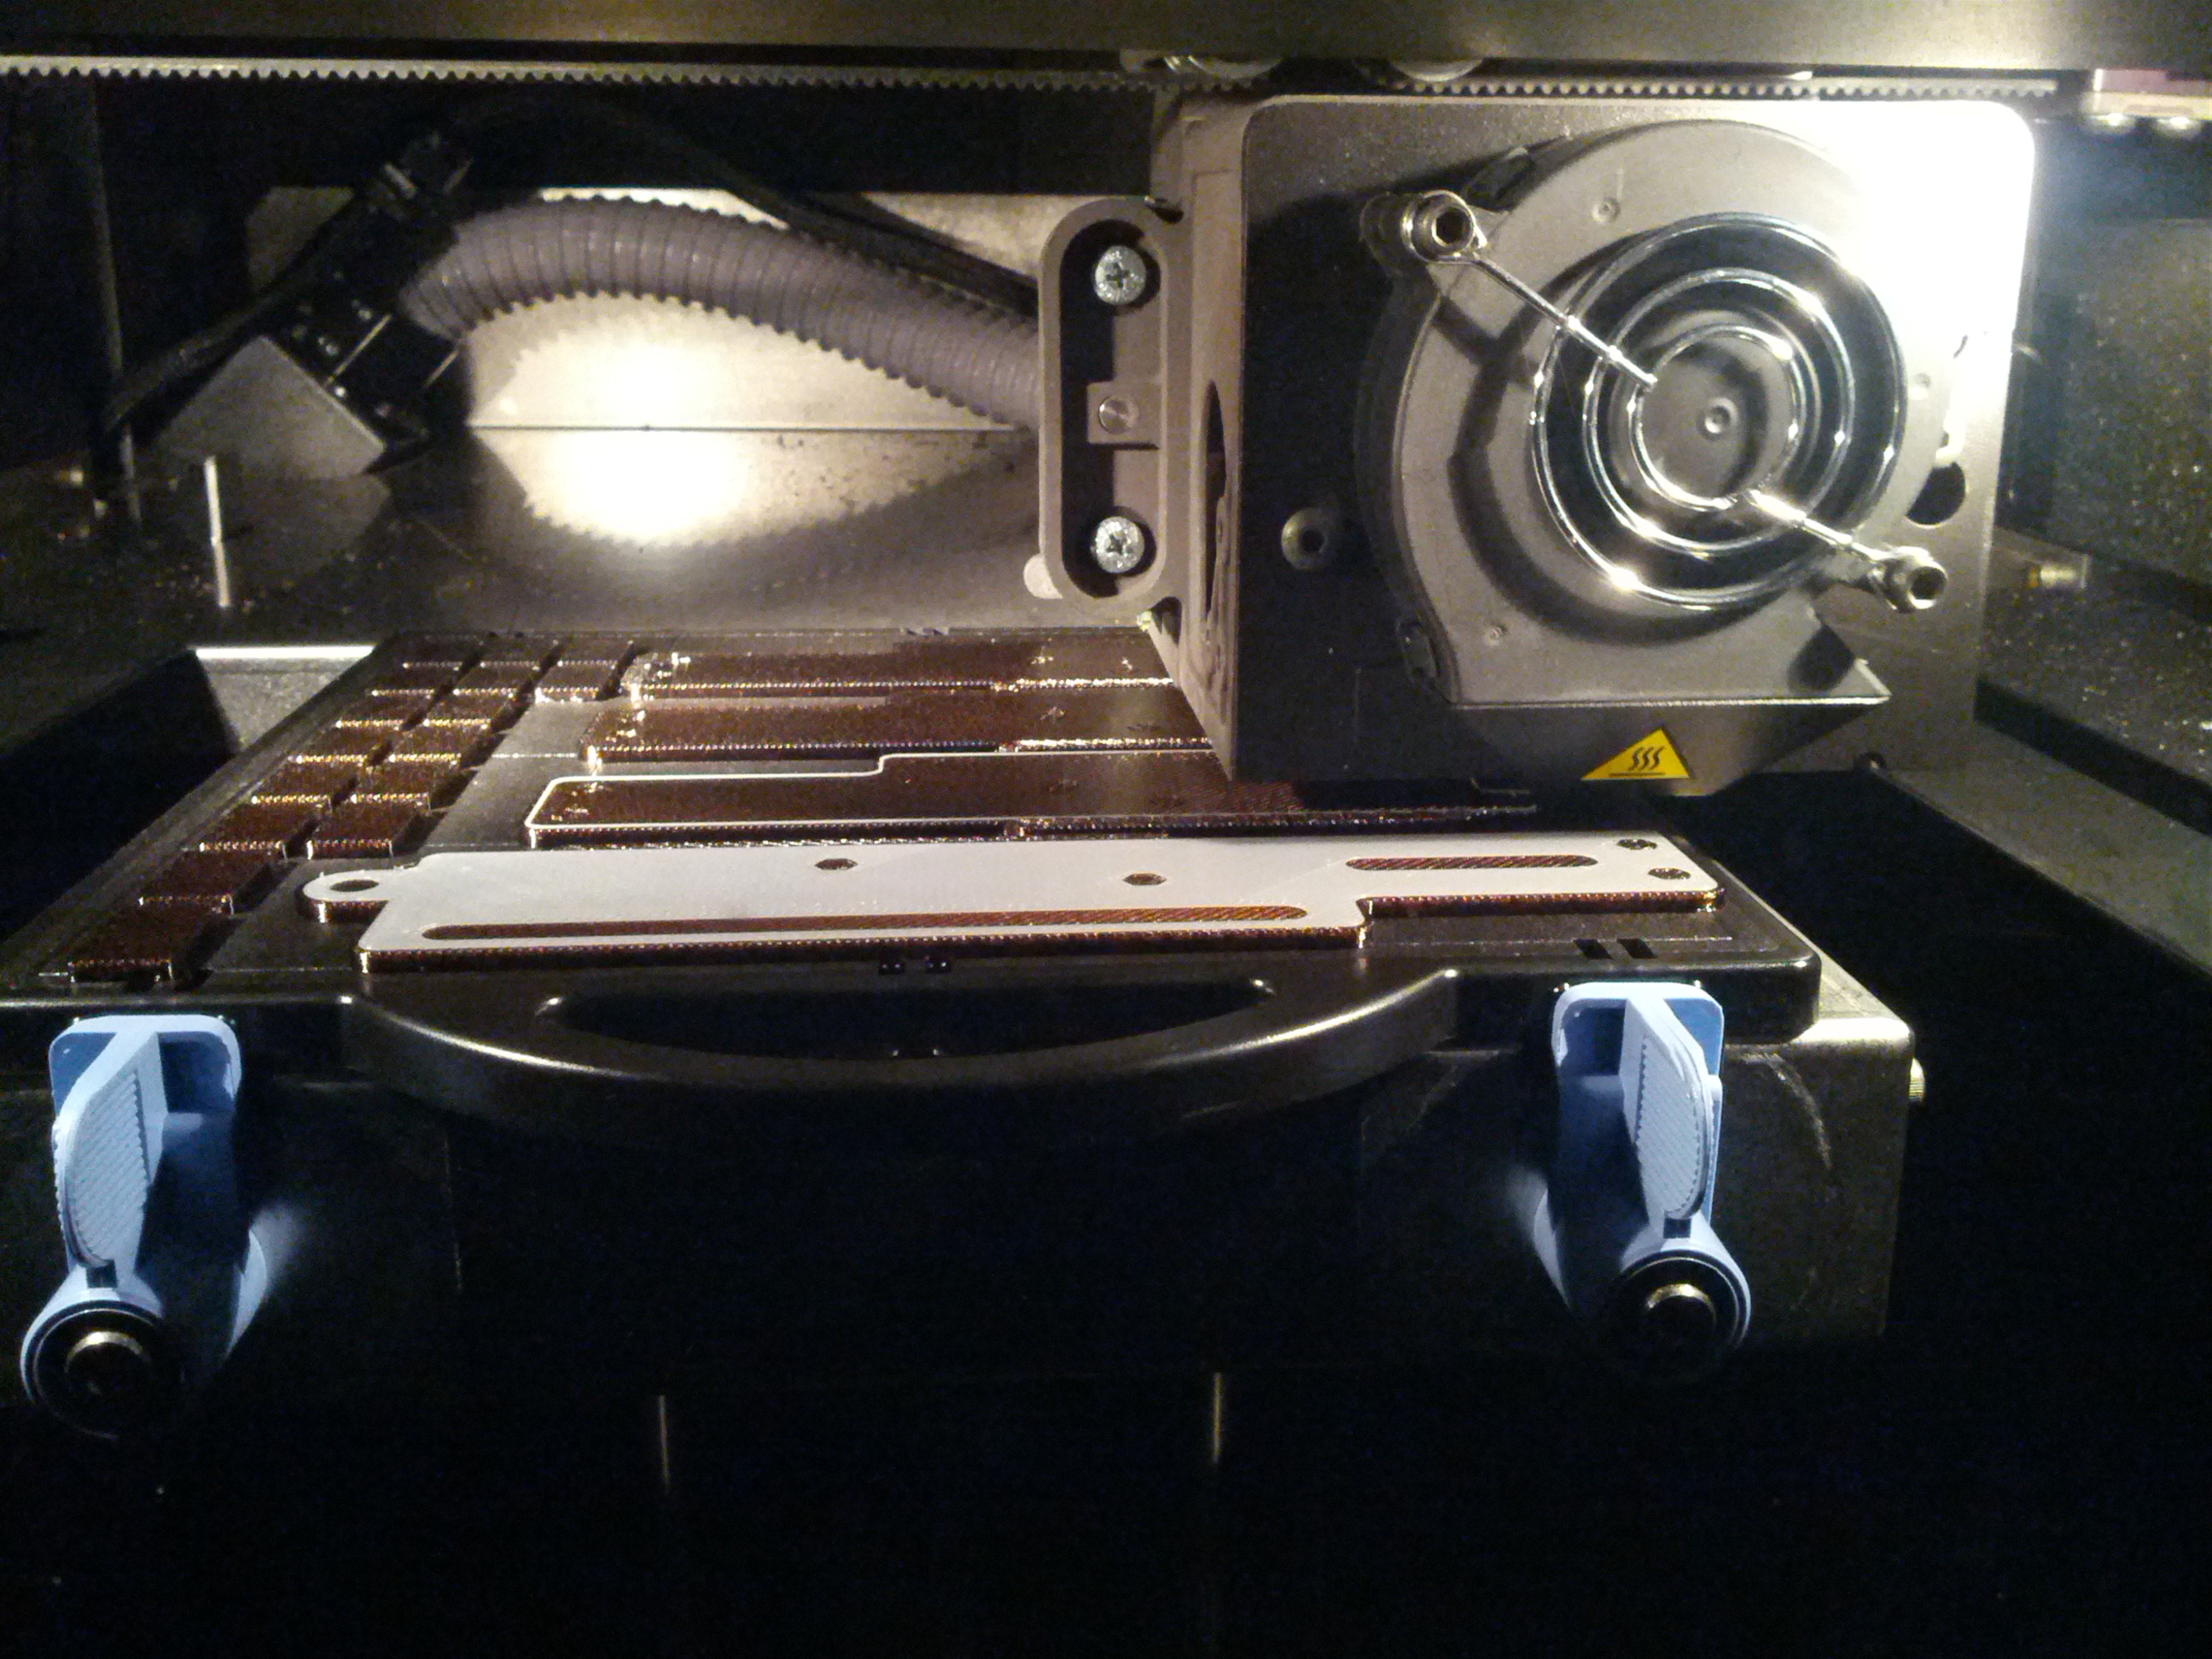
\includegraphics[width=0.8\linewidth]{img/pic/IMG_20140530_184940.jpg}\\
%  \vspace{0.5cm}
%  \end{center}
%\end{frame}
\begin{frame}[c]
    \frametitle{Distribution in the field cage}
  \begin{center}
  	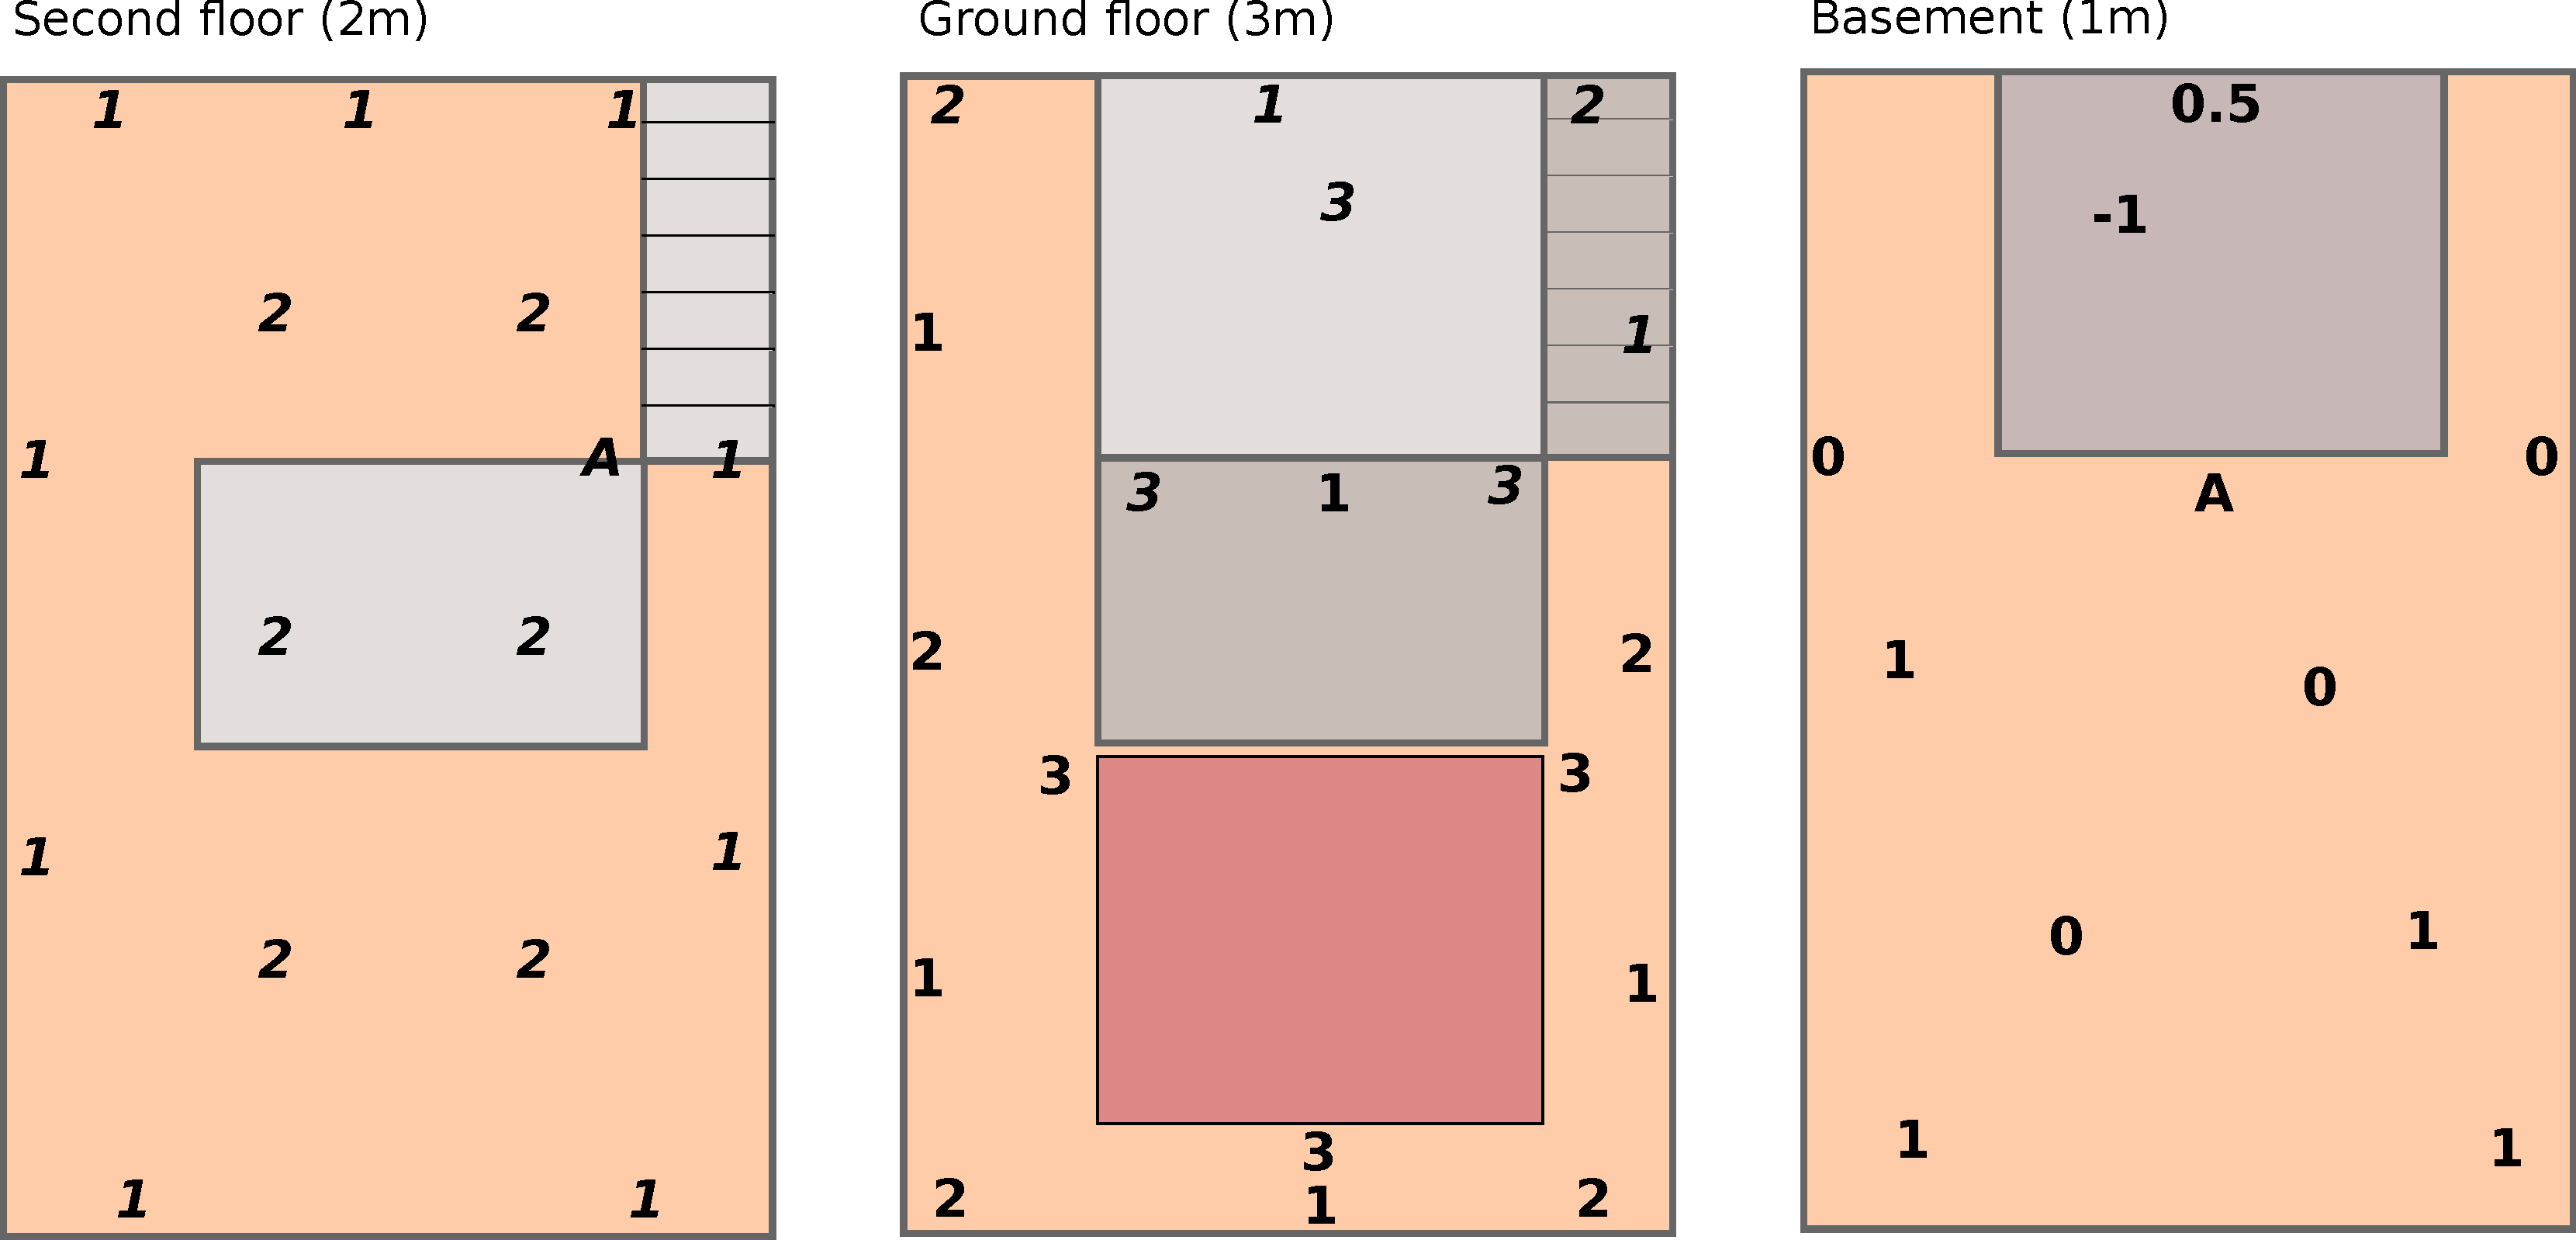
\includegraphics[width=0.9\linewidth]{img/installPlan.pdf}\\
  \vspace{0.5cm}
  \end{center}
\end{frame}
\begin{frame}[c]
    \frametitle{Improvements}
		\begin{alertblock}{Problems}
			\textcolor{blue!30!green}{
				\begin{itemize}
					\item DHCP
					\item DNS
					\item Cases
				\end{itemize}
			}
		\end{alertblock}
\end{frame}
\end{document}
